\chapter{Macroprogramming IoT Systems with Large Language Models}
\label{chap:language-based-macroprogramming}

% NOTE: this chapter develops one publication: "A Language-based Approach to
% Macroprogramming for IoT Systems through Large Language Models" (ACM Trans.
% Internet Things 6(4), 2025, doi 10.1145/3758326, key
% DBLP:journals/tiot/AguzziFV25). Code-generation background is given locally;
% fields, alignment, and self-stabilisation are covered by
% \cref{subsec:aggregate-computing}.
% Deliberately not reproduced: the paper's survey of macroprogramming paradigms,
% covered by \cref{sec:macro-programming}; its per-test-case result tables and
% the full sixteen-model matrix, summarised and cited instead. The scenario is
% \cityevt's crowding requirement from \cref{sec:multiparty-motivation} rather
% than a second one, since the paper's marathon case is the same problem.

Macroprogramming lets a developer describe collective behaviour in a single program.
Writing that program requires knowledge of the language's distributed operations:
for example, how devices retain state, exchange values with neighbours, and compose those operations into coordination patterns.
This chapter examines whether a natural-language task description can be translated into an aggregate program in ScaFi.
It addresses the program-generation part of \cref{rq:languages}.

The approach supplies an \ac{LLM} with a \emph{body of knowledge}:
a short manual of ScaFi operators, illustrated by programs and their outputs over successive rounds.
The manual is included in the prompt, without fine-tuning the model or modifying its decoder.
The evaluation compares sixteen models at three knowledge levels and checks the generated programs by compilation and simulation~\cite{DBLP:journals/tiot/AguzziFV25}.

\section{Code Generation for Domain-Specific Languages}
\label{sec:llms-for-code-generation}

\Acp{LLM} trained on source code can generate programs from descriptions of intended behaviour or from examples.
The 2021 Codex study evaluated this capability on HumanEval,
a benchmark of hand-written Python problems scored by whether generated functions pass their accompanying unit tests.
The model, pretrained on public source code and fine-tuned on function-body examples,
solved 28.8\% of the problems.
The study introduced test-based evaluation through \emph{pass@k} and described the model behind the initial version of GitHub Copilot~\cite{DBLP:journals/corr/abs-2107-03374}.

Specialised \acp{DSL} may have few examples in a model's training corpus.
A model can therefore reproduce the syntax of a host language such as Scala while misusing the operations of an embedded DSL.
It may also invent constructs or import syntax from other languages.
Both syntactic validity and the meaning of domain-specific operations need to be addressed.

\emph{Constrained decoding} restricts the tokens available at each generation step to those permitted by constraints on the output.
PICARD incrementally parses generated SQL and rejects tokens that cannot be completed into a valid query~\cite{DBLP:conf/emnlp/ScholakSB21}.
Synchromesh combines checks on partial programs with retrieval of semantically relevant examples~\cite{DBLP:conf/iclr/PoesiaP00SMG22}.
Grammar-constrained decoding applies a target grammar to structured-output tasks, including code generation, without retraining the model for each language~\cite{DBLP:conf/emnlp/GengJP023}.
These methods enforce the constraints supplied to the decoder; syntactic constraints alone do not establish the intended behaviour of a program.

\emph{Grammar prompting} supplies each example together with the subset of the target grammar needed to produce it.
The model first predicts a specialised grammar for the task and then generates a program under its rules.
This allows an off-the-shelf model to work with a DSL on which it has not been fine-tuned~\cite{DBLP:conf/nips/WangW0CSK23}.

The approach studied here supplies operational examples of aggregate computation in the prompt~\cite{DBLP:journals/tiot/AguzziFV25}.
The examples explain what values an operator produces at each device over time.
This information is needed to distinguish field operations from sequential operations with similar syntax.
Compilation checks the resulting program's syntax and types; simulation checks its behaviour against task-specific assertions.

\section{Aggregate Programs from Natural-Language Specifications}
\label{sec:llm-macroprogramming-motivation}

Aggregate computing provides a global specification of collective behaviour from which each device's computation is derived.
A domain expert can describe an intended collective outcome without prescribing every local interaction.
The field calculus provides a general computational basis:
its space-time universality covers computable functions over space-time event structures~\cite{DBLP:conf/coordination/AudritoBDV18}.

Generated programs use the same execution model as hand-written aggregate programs.
When they satisfy the composition conditions of self-stabilising building blocks, they inherit the corresponding convergence guarantees~\cite{DBLP:journals/tomacs/ViroliABDP18}.
Similarly, the deployment-independence result of \cref{thm:deployment-independence} applies when the generated program's decomposition and deployment satisfy its hypotheses.
The method of producing a program does not establish these properties by itself.

\subsection{Crowding-Monitor Requirements}
\label{subsec:llm-crowding-task}

The crowding monitor in \cityevt (\cref{sec:multiparty-motivation}) estimates crowd density around each participant and reports areas above a threshold.
Its requirements provide a task for program generation:
density is estimated from proximity between participants' phones,
never from their positions,
and an alert has to reach the region around a crowded area rather than the whole system.
%
A non-expert states the task in one sentence --
mark the areas where devices are packed more densely than a threshold, and tell every device how far it is from the nearest such area.
%
Implementing this description in ScaFi requires knowing that neighbour counting is a fold over the neighbourhood,
that the fold has a variant excluding the device itself,
and that distance-to-a-region is a gradient rather than a broadcast.

The body of knowledge supplies examples of these operations.

\subsection{Program Generation Before Deployment}
\label{subsec:llm-positioning}

Work on LLM-based orchestration uses a model at run time to interpret sensor data and issue commands~\cite{DBLP:journals/diot/ZongHGLK25}.
Here, the model is used before deployment to produce a program.
The aggregate runtime then executes that program without invoking the model.
Developers can inspect, type-check, and simulate the generated artefact before it runs on physical devices.

Three questions organise what follows:
whether a current general-purpose model produces valid aggregate code when given nothing but the task;
whether prompting alone can convey the paradigm's temporal abstractions,
its spatial ones,
and the spatio-temporal ones that compose both;
and whether a model that has been given the vocabulary composes it into solutions it was not shown.

\section{Body of Knowledge for ScaFi}
\label{sec:body-of-knowledge}

The \emph{body of knowledge} is a short operational manual of ScaFi's field operators and self-organising building blocks~\cite{casadei2022scafi}.
It describes their use through executable examples and traces of the values produced over successive rounds.
The manual is placed in the model's context when a program is generated.

\subsection{Operator Descriptions and Execution Traces}
\label{subsec:bok-structure}

The body of knowledge is a sequence of entries,
each adding one operator on top of those already introduced.
%
An entry has three slots:
a one-line scenario saying what problem the operator solves,
the operator's signature with its parameters named,
and a minimal program using it together with the values that program produces over successive rounds.
%
\Cref{lst:bok-entry} is the entry for temporal evolution,
the first one in the sequence.

\noindent\begin{minipage}{\linewidth}
\begin{lstlisting}[
  numbers=none,
  frame=single,
  captionpos=b,
  basicstyle=\ttfamily\scriptsize,
  caption={The body-of-knowledge entry for temporal evolution.},
  label={lst:bok-entry},
]
# Temporal Evolution allows devices to maintain and update state over time #

# The rep construct allows stateful computation:
def rep[A](init: => A)(evolve: A => A): A
- init: The initial value
- evolve: Function that takes the current value and returns the next value

# Example: Creating a counter that increases by 1 each round
def main(): Int = rep(0)(_ + 1)
When executed repeatedly:
Round 1: 0
Round 2: 1
Round 3: 2
\end{lstlisting}
\end{minipage}

The trace shows the values produced at each device over successive rounds.
For \code{rep}, it illustrates how each device retains and updates its own state.

The manual covers the operators in \cref{tab:scafi-operators}.
It first introduces sensing, local state, neighbourhood interaction, and conditionals,
then combines them through the self-organising building blocks.
The evaluation compares three knowledge levels:
no manual, the core operators alone, and the core together with the building blocks.
This comparison tests whether examples of higher-level patterns improve generation beyond examples of the individual operators.

\subsection{Expert-guided Refinement}
\label{subsec:bok-codesign}

The body of knowledge is refined iteratively:
the current version is used to generate code for the test cases,
an expert reads the failures,
and the entry that would have prevented each failure is added or rewritten.
%
The expert is shown the four things needed to diagnose a failure --
the body of knowledge used, the task, the code the model produced, and the reference program --
and answers a single question: which concept was misunderstood.

Entries address observed failures, keeping the manual focused on the concepts used by the tasks.
%
One constraint governs what may be added: an entry must raise the abstraction available to the model without containing the solution to a test case.
%
An entry showing how to compute a gradient is legitimate;
an entry showing how to compute a gradient that avoids obstacles is not,
because a test case asks for exactly that.
%
Automating the loop is conceivable,
by treating the body of knowledge as a parameter optimised against test outcomes.
%
Expert review is needed to keep operator examples separate from solutions to the evaluation tasks.

\section{Generation and Validation}
\label{sec:llm-pipeline}

\Cref{fig:llm-pipeline} shows how the expert's work and the practitioner's fit together.
%
On the left, an expert refines the body of knowledge against test cases;
on the right, a practitioner writes a task in natural language and receives a program.
%
The left side is done once, by someone who knows the paradigm;
the right side is done by someone who does not.

\begin{figure}[t]
    \centering
    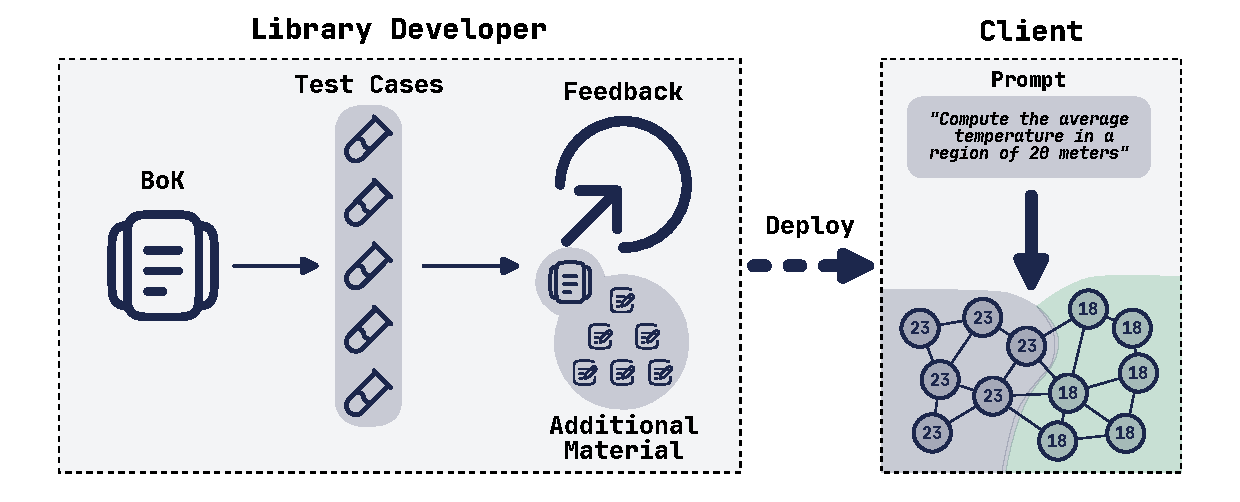
\includegraphics[width=\textwidth]{llm-pipeline.pdf}
    \caption[Generating aggregate programs from natural language]{Generating aggregate programs from natural language. The body of knowledge is refined against test cases by an expert (left) and then used, unchanged, to answer a practitioner's task description (right). Adapted from~\cite{DBLP:journals/tiot/AguzziFV25}.}
    \label{fig:llm-pipeline}
\end{figure}

\subsection{Prompt Template}
\label{subsec:llm-prompt}

The prompt template is fixed across every model, task, and knowledge level,
so the only things that vary between runs are the body of knowledge and the task.
%
\Cref{lst:prompt-template} gives it in full.

\noindent\begin{minipage}{\linewidth}
\begin{lstlisting}[
  numbers=none,
  frame=single,
  captionpos=b,
  basicstyle=\ttfamily\scriptsize,
  caption={The prompt template. Only the two placeholders vary between runs.},
  label={lst:prompt-template},
]
You are an expert in Aggregate Computing and the ScaFi programming language.
I will give you a programming task, and you should provide a solution in ScaFi.

Body of Knowledge:
{BOK}

TASK:
{TASK_DESCRIPTION}

FORMAT REQUIREMENTS:
- Return ONLY a single ScaFi function with signature "def main(): Any"
- Do not include explanations, comments, or additional text
- Ensure the code is syntactically valid and correctly implements the
  requested behavior

Your answer:
\end{lstlisting}
\end{minipage}

The required shape, \code{def}\;\code{main(): Any}, lets the evaluation harness compile each response without manual editing.
Responses that violate the format are recorded as failures.

\subsection{Test Cases}
\label{subsec:llm-test-cases}

A test case has four parts.
%
The task description is the natural-language text substituted into the prompt.
%
The reference program, written by an expert, fixes what correct behaviour is, and is itself run to confirm that the assertions are satisfiable.
%
The initial state is a network graph whose nodes are devices carrying positions, sensor values, and identifiers, and whose edges are communication links.

The fourth part is a set of assertions.
These check local values at named devices,
but they also check emergent properties of the whole field --
that a gradient's values increase with distance from the source, that every device in a region agrees on its region's average --
and they are evaluated only after enough rounds for the computation to stabilise.
%
Assertions check behaviour over the observation period; a transient correct value is insufficient.

\subsection{Compilation, Simulation, and Deployment}
\label{subsec:llm-validation}

Validation has three stages.
%
The ScaFi compiler rejects what is not syntactically valid or not well typed,
and catches the API calls a model invents.
%
Simulation in Alchemist (\cref{subsec:cas-platforms}) runs the program over a configured network and checks its emergent behaviour against the assertions~\cite{DBLP:journals/jos/PianiniMV13}.
%
Deployment then places it on real infrastructure, with monitoring in place,
since neither of the first two stages says anything about conditions the simulation did not reproduce.

\section{Evaluation}
\label{sec:llm-evaluation}

\subsection{Setup and Metrics}
\label{subsec:llm-setup}

Eleven test cases were built, in three groups.
%
Five exercise either time or space, not both:
counting down from a fixed value, which needs only \code{rep};
counting neighbours, in two variants, one counting the device itself and one not;
gathering neighbours' identifiers;
and computing the minimum distance to a neighbour.
%
Three require time and space at once:
the maximum identifier over the whole network,
the gradient from a source,
and the same gradient with obstacles to route around.
%
Three are stated at the level of the building blocks:
a channel between a source and a destination,
the same channel with obstacles,
and an area-wise alarm that partitions the network into regions and raises an alert in any region whose average temperature exceeds a threshold.

Sixteen models were run against all eleven cases at each of the three knowledge levels,
twenty times per combination,
with the reference programs run alongside as a control~\cite{DBLP:journals/tiot/AguzziFV25}.
%
Two metrics summarise the outcome.
%
\emph{pass@k} estimates the probability that at least one of $k$ sampled programs compiles and passes the assertions.
%
\emph{compile@k} estimates the probability that at least one of $k$ sampled programs compiles.
The gap between the two measures separates compilation success from success on the behavioural assertions.

\subsection{Effect of the Body of Knowledge}
\label{subsec:llm-results}

\Cref{tab:llm-pass-rates} reports seven representative models;
\cref{fig:llm-knowledge-improvement} shows the same three levels for ten of the sixteen, together with their average.

\begin{table}[t]
    \centering
    \small
    \caption[Pass and compile rates by knowledge level]{Pass and compile rates at $k=10$ for seven representative models, at the three knowledge levels. Data from~\cite{DBLP:journals/tiot/AguzziFV25}, which reports all sixteen models and $k \in \{1, 5, 10\}$.}
    \label{tab:llm-pass-rates}
    \setlength{\tabcolsep}{4pt}
    \begin{tabular}{@{}lcccccc@{}}
        \toprule
        & \multicolumn{2}{c}{\textbf{No knowledge}} & \multicolumn{2}{c}{\textbf{Core operators}} & \multicolumn{2}{c}{\textbf{+ Building blocks}} \\
        \cmidrule(lr){2-3} \cmidrule(lr){4-5} \cmidrule(lr){6-7}
        \textbf{Model} & pass@10 & comp@10 & pass@10 & comp@10 & pass@10 & comp@10 \\
        \midrule
        Gemini 2.5 Pro      & 0.50 & 0.77 & 0.73 & 0.99 & 0.84 & 1.00 \\
        Gemini 2.0 Flash    & 0.07 & 0.07 & 0.71 & 0.91 & 0.86 & 0.95 \\
        Claude 3.7 Sonnet   & 0.17 & 0.62 & 0.80 & 1.00 & 0.79 & 1.00 \\
        GPT-4.1 Mini        & 0.13 & 0.45 & 0.61 & 0.99 & 0.61 & 0.94 \\
        Llama 3.3 70B       & 0.00 & 0.11 & 0.75 & 0.97 & 0.61 & 0.80 \\
        Llama 4 Maverick    & 0.00 & 0.05 & 0.55 & 0.90 & 0.50 & 0.80 \\
        Mistral 8B          & 0.00 & 0.42 & 0.00 & 0.90 & 0.05 & 0.90 \\
        \bottomrule
    \end{tabular}
\end{table}

\begin{figure}[t]
    \centering
    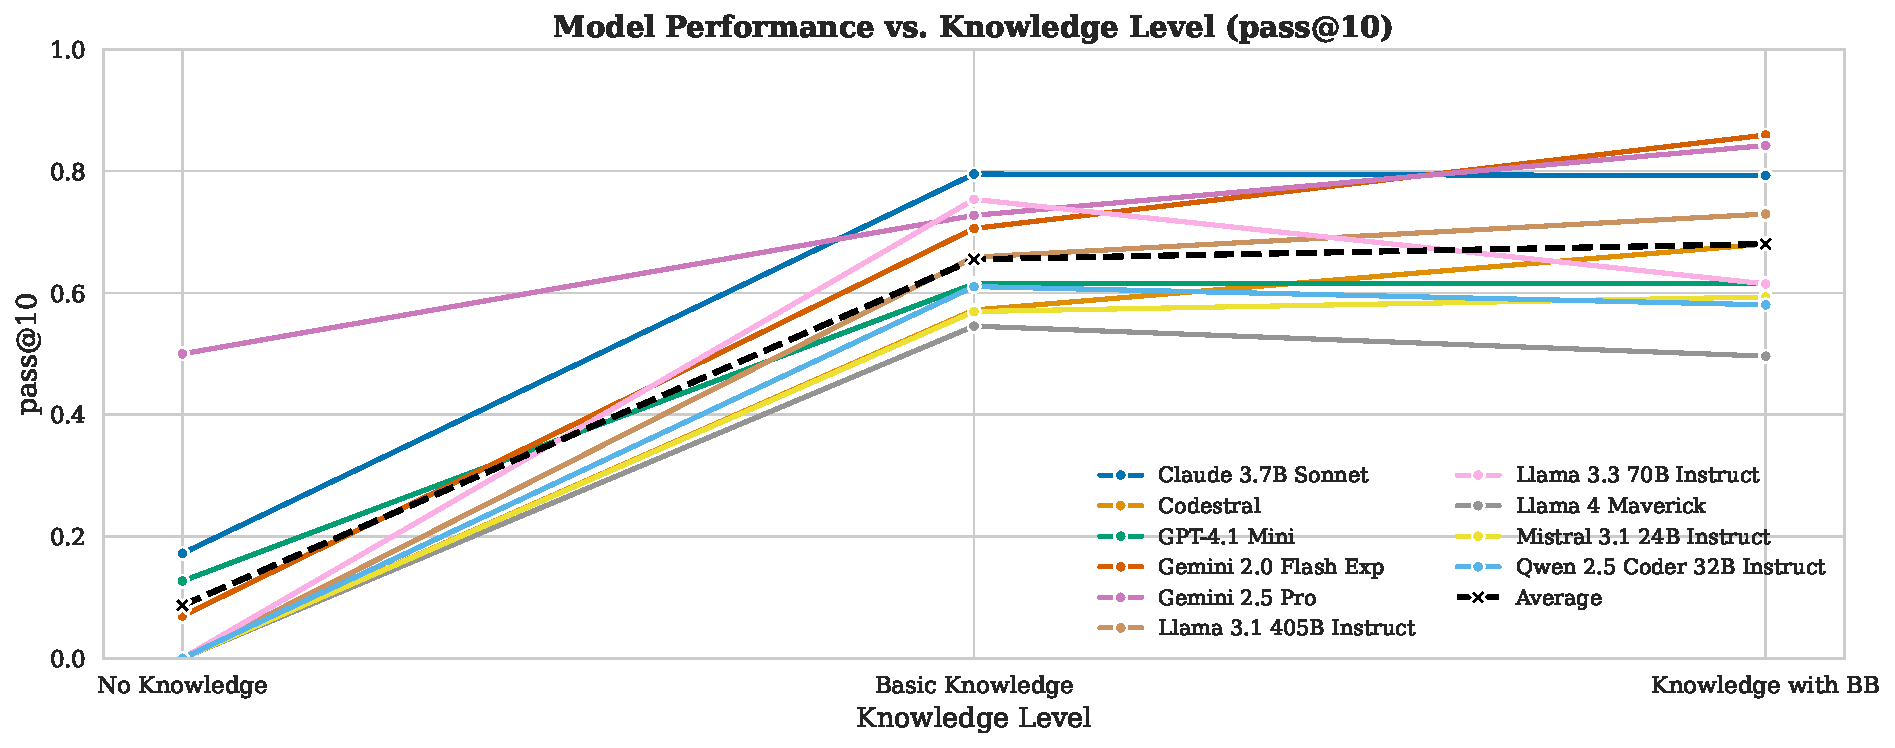
\includegraphics[width=\textwidth]{llm-knowledge-improvement.pdf}
    \caption[Pass rate against knowledge level]{Pass rate at $k=10$ against knowledge level. The effect of supplying core operators and building blocks varies across models. Data from~\cite{DBLP:journals/tiot/AguzziFV25}.}
    \label{fig:llm-knowledge-improvement}
\end{figure}

Without a body of knowledge, most models failed to generate working aggregate programs.
%
Twelve of the sixteen models never pass a single test case at any $k$,
and the failures are dominated by code that does not compile:
compile@10 is 0.11 for Llama 3.3 70B and 0.05 for Llama 4 Maverick.
%
Two of the four exceptions stand out.
%
Gemini 2.5 Pro passes half the cases at $k=10$, and Claude 3.7 Sonnet a sixth.
%
Successful gradient attempts reproduce the canonical formulation,
\code{rep} over a \code{mux} on the source sensor with \code{minHoodPlus} of the neighbours' distances.
%
These successes alone do not establish which aggregate-computing material was present in the training data.

Supplying the core operators improves compilation rates across models.
%
Compile rates rise in every case, most of them into the nineties:
GPT-4.1 Mini goes from 0.45 to 0.99,
Claude 3.7 Sonnet from 0.62 to 1.00.
%
Pass rates follow, but by less.
%
Of the twelve models that were at zero, nine end between 0.45 and 0.75;
the remaining three stay below 0.30, and Mistral 8B never rises above 0.05 at any level.
%
These gains were obtained by adding the manual to the prompt.
Gemini 2.5 Pro, which already passed half the cases without the manual, improves from 0.50 to 0.73.

Adding the building blocks does not continue the trend.
%
The two Gemini models gain another 11 and 15 points of pass@10,
and Gemini 2.5 Pro reaches 0.76 on the channel with obstacles and 0.70 on the area-wise alarm,
the two tasks on which the core-operator level left every model weak.
%
Two models move the other way:
Llama 3.3 70B falls from 0.75 to 0.61, and its compile rate from 0.97 to 0.80;
Llama 4 Maverick falls from 0.55 to 0.50.
%
Claude 3.7 Sonnet stays where it was.
%
The failures at this level include unnecessary uses of \code{G} for tasks expressible with \code{foldhood} over \code{nbr}.
Additional abstractions can introduce errors when a model selects an unsuitable building block.

\subsection{Semantic Errors in Generated Programs}
\label{subsec:llm-failure-modes}

Two semantic errors recur across models even with the full body of knowledge.

One is reading \code{nbr} as a collection.
%
\Cref{lst:nbr-misuse} is a gradient attempt from Gemini 2.0 Flash that compiles and is wrong.

\noindent\begin{minipage}{\linewidth}
\begin{lstlisting}[
  style=scala3,
  escapeinside={(*@}{@*)},
  caption={A gradient in which \texttt{nbr} is mistaken for a collection.},
  label={lst:nbr-misuse},
]
rep[Option[Double]](
  if (sense[Boolean]("source")) Some(0.0) else None
) { distance =>
  mux(distance.isDefined && !sense[Boolean]("obstacle")) {
    minHood(nbr(distance).map(_ + nbrRange()))(*@\label{line:nbr-map}@*)
  } { distance }
}.getOrElse(Double.PositiveInfinity)
\end{lstlisting}
\end{minipage}

The \code{map} on \cref{line:nbr-map} operates on the local \code{Option} value.
%
\code{nbr(distance)} does not return the neighbours' distances as a collection to be traversed;
it causes the surrounding expression to be evaluated once per aligned neighbour,
and \code{minHood} folds those evaluations.
%
Treating this value as a collection of neighbours confuses Scala's local operations with ScaFi's neighbourhood evaluation.

The other is using \code{branch} where \code{mux} is meant,
as in \cref{lst:branch-misuse}.

\noindent\begin{minipage}{\linewidth}
\begin{lstlisting}[
  style=scala3,
  escapeinside={(*@}{@*)},
  caption={A gradient whose conditional separates source and non-source evaluation domains.},
  label={lst:branch-misuse},
]
rep(Double.MaxValue) { dist =>
  branch(sense[Boolean]("source")) { 0.0 } {
    minHood(nbr(dist) + nbrRange())
  }
}
\end{lstlisting}
\end{minipage}

The code assigns zero to sources and computes a neighbourhood minimum elsewhere.
However, \code{branch} evaluates these expressions in separate domains.
The minimum at a non-source device therefore excludes source devices, even when they are physical neighbours, and the gradient never forms.
%
\code{mux} evaluates both arms and selects between the values, leaving alignment intact.

Both errors have the same shape.
%
The model applies the sequential reading of a construct whose field reading is different,
and nothing in the syntax signals the difference.
%
Traces of values at each device over successive rounds help expose these differences in meaning.

\subsection{Generated Compositions of Building Blocks}
\label{subsec:llm-novelty}

The third question was whether a model given the vocabulary composes it into something it was not shown.
%
Two results from Gemini 2.5 Pro show that it does.

The first is the channel with obstacles.
%
The body of knowledge builds channels the standard way,
from gradients,
and handles regions to avoid with \code{branch}.
%
The generated solution does neither.
%
It builds a potential with \code{G} and then uses the collect cast \code{C} to propagate a boolean back from the destination along that potential,
which marks the connecting region without computing a second gradient.
%
It avoids obstacles by returning an infinite value from the metric at obstacle devices,
so the potential routes around them by construction.
%
Neither move appears in the manual.

The second result reconstructs a pattern that has a name in the literature.
%
\Cref{lst:scr-rediscovery} is the model's answer to the area-wise alarm.

\noindent\begin{minipage}{\linewidth}
\begin{lstlisting}[
  style=scala3,
  escapeinside={(*@}{@*)},
  caption={The area-wise temperature alarm, as generated with the building blocks available.},
  label={lst:scr-rediscovery},
]
val isLeader = S(2, nbrRange)(*@\label{line:scr-leader}@*)
val temperature = sense[Double]("temperature")
val potential = G(isLeader, 0.0, _ + nbrRange(), nbrRange)(*@\label{line:scr-potential}@*)
val areaTemperature = C[Double, Double](potential, _ + _, temperature, 0.0)
val areaSize = C[Double, Int](potential, _ + _, 1, 0)(*@\label{line:scr-collect}@*)
val averageTemperature =
  if (areaSize > 0) areaTemperature / areaSize else 0.0
val alarm = averageTemperature > 30.0
G(isLeader, alarm, (a: Boolean) => a, nbrRange)(*@\label{line:scr-broadcast}@*)
\end{lstlisting}
\end{minipage}

This is the self-organising coordination regions pattern~\cite{DBLP:journals/fgcs/PianiniCVN21}.
%
Leaders are elected at a fixed grain (\cref{line:scr-leader}),
a potential from each leader defines its region (\cref{line:scr-potential}),
two collect casts bring the sum and the count of the region's readings to its leader (\cref{line:scr-collect}),
and the leader's decision is cast back over the same region (\cref{line:scr-broadcast}).
%
The pattern was not in the body of knowledge;
only the three blocks it is made of were.
%
With the core operators alone, no model produced a working solution for this task,
whereas providing the building blocks enabled this composition.

\subsection{Crowding-Monitor Simulation}
\label{subsec:llm-case-study}

The crowding-monitor task tests the generated program on a mobile network.
%
\Cref{lst:crowding-monitor} is what the best-performing model produced for it.

\noindent\begin{minipage}{\linewidth}
\begin{lstlisting}[
  style=scala3,
  escapeinside={(*@}{@*)},
  caption={The generated crowding monitor: local density, then distance to the nearest crowded area.},
  label={lst:crowding-monitor},
]
val DENSITY_THRESHOLD_COUNT = 50
val localNeighboringDeviceCount = foldhoodPlus(0)(_ + _)(nbr(1))(*@\label{line:crowd-count}@*)
val isLocallyOvercrowded =
  localNeighboringDeviceCount >= DENSITY_THRESHOLD_COUNT
G[Double](
  source = isLocallyOvercrowded,(*@\label{line:crowd-source}@*)
  field  = 0.0,
  acc    = pathDistanceSoFar => pathDistanceSoFar + nbrRange(),
  metric = nbrRange
)
\end{lstlisting}
\end{minipage}

The program is the two-part decomposition the task calls for.
%
\Cref{line:crowd-count} estimates local density by folding a constant over the neighbourhood,
using the \code{foldhoodPlus} variant so a device does not count itself.
%
The estimate rests on proximity and needs no positions,
so the privacy constraint of \cref{sec:multiparty-motivation} is met by the choice of operator rather than by a separate mechanism.
%
The gradient cast from \cref{line:crowd-source} then turns the boolean field of overcrowded devices into a distance field,
so every device knows how far the nearest crowded area is
and an alert can be scoped to the devices whose distance is below a given bound.

The program was run in Alchemist on mobility traces from a city marathon,
with about 300 mobile devices, realistic movement, and modelled Bluetooth propagation~\cite{DBLP:journals/computer/BealPV15}.
%
Crowded areas are identified as they form,
the distance field propagates the information into the surrounding region,
and both track the crowd as participants move.
%
The full sequence of simulation snapshots is in the original evaluation~\cite{DBLP:journals/tiot/AguzziFV25}.

\section{Discussion}
\label{sec:llm-macroprogramming-discussion}

Providing operational examples improved the generation of aggregate programs in this evaluation.
With the core operators, models that produced no usable programs without the manual solved most of the tasks.
For the strongest models, adding the building blocks enabled solutions to more complex tasks and the composition of a published pattern absent from the manual.
Model size alone did not explain performance:
Llama 3.1 405B led at no knowledge level and, with the core operators, obtained a pass@10 of 0.66 against Llama 3.3 70B's 0.75.
The experiment does not establish how differences in pretraining data contributed to these results.

The manual was supplied through prompting, without fine-tuning or constrained decoding.
Its examples address the meaning of field operations.
The failures in \cref{subsec:llm-failure-modes} show why syntactic constraints alone are insufficient:
a program may compile while applying a field operator incorrectly.
Behavioural assertions remain necessary alongside compilation.

Three limitations affect the interpretation of the results.
The body of knowledge was refined against the same test cases used in the evaluation,
so the reported rates measure performance within that task family.
Transfer to independent tasks requires a separate evaluation.
\emph{pass@k} measures satisfaction of assertions, which provides limited evidence of correctness and does not measure efficiency:
a passing program may be expensive to evaluate or may satisfy incomplete assertions accidentally.
Finally, the reported ranking applies to the model versions tested and may change as hosted models are updated.
Simulation checks behaviour only under the tested conditions, so deployment also requires monitoring under the conditions of use.
